\documentclass[
	fontsize=12pt,
	paper=a4,
	numbers=noenddot,
	parskip=half,
	openany
]{scrbook}
\usepackage{tcolorbox}

\include{../../../for_latex/preamble}
% ##################################################
% Gemeinsames Setup fuer die Probeklausuren
% (Java-Listings, Hinweis-/Beispiel-Boxen, Struktogramm-Stile in TikZ)
% wird nach \include{../for_latex/preamble} per \input eingebunden
% ##################################################

% --- Java Code-Highlighting ---
\definecolor{codegray}{rgb}{0.5,0.5,0.5}
\definecolor{codepurple}{rgb}{0.58,0,0.82}
\definecolor{backcolour}{rgb}{0.95,0.95,0.92}
\definecolor{keywordcolor}{rgb}{0.8,0.47,0.13}

\lstdefinestyle{javastyle}{
	backgroundcolor=\color{backcolour},
	commentstyle=\color{codegray},
	keywordstyle=\color{keywordcolor}\bfseries,
	numberstyle=\tiny\color{codegray},
	stringstyle=\color{codepurple},
	basicstyle=\ttfamily\footnotesize,
	breakatwhitespace=false,
	breaklines=true,
	captionpos=b,
	keepspaces=true,
	numbers=left,
	numbersep=5pt,
	showspaces=false,
	showstringspaces=false,
	showtabs=false,
	tabsize=2,
	language=Java,
	frame=single,
	rulecolor=\color{black!30}
}

\lstset{style=javastyle}

% --- Hinweis-/Beispiel-/Formel-Umgebungen (schlicht, ohne farbige Box) ---
\newenvironment{hinweis}[1][Hinweis]%
	{\par\smallskip\noindent\textbf{#1.}\enspace\ignorespaces}%
	{\par\smallskip}

\newenvironment{beispiel}[1][Beispiel]%
	{\par\smallskip\noindent\textbf{#1:}\par\nobreak\vspace{2pt}}%
	{\par\smallskip}

\newenvironment{formeln}[1][Gegebene Formeln]%
	{\par\smallskip\noindent\textbf{#1:}\par\nobreak\vspace{2pt}}%
	{\par\smallskip}

% ##################################################
% Struktogramm (Nassi-Shneiderman) in reinem TikZ
% ##################################################
\newlength{\nswidth}\setlength{\nswidth}{11.5cm}   % Gesamtbreite
\newlength{\nsind}\setlength{\nsind}{0.55cm}        % Einrueckung je Schleifenebene
% vorberechnete Versatzbreiten fuer Verzweigungen (in Koordinaten nutzbar)
\newlength{\nshalf}\setlength{\nshalf}{\dimexpr\nswidth/2\relax}            % halbe Gesamtbreite
\newlength{\nshalfi}\setlength{\nshalfi}{\dimexpr(\nswidth-\nsind)/2\relax}  % halbe Breite, 1x eingerueckt
\newlength{\nshalfii}\setlength{\nshalfii}{\dimexpr(\nswidth-2\nsind)/2\relax} % halbe Breite, 2x eingerueckt

\tikzset{
	% Basis fuer Anweisungs-/Verzweigungsbloecke
	nb/.style={draw, line width=0.4pt, anchor=north west, inner sep=4pt,
		align=left, font=\footnotesize, fill=white, minimum height=0.8cm},
	% volle Breite
	nbfull/.style={nb, minimum width=\nswidth,
		text width=\dimexpr\nswidth-8pt\relax},
	% eine Ebene eingerueckt (Schleifenrumpf)
	nbi/.style={nb, minimum width=\dimexpr\nswidth-\nsind\relax,
		text width=\dimexpr\nswidth-\nsind-8pt\relax},
	% zwei Ebenen eingerueckt (Schleife in Schleife)
	nbii/.style={nb, minimum width=\dimexpr\nswidth-2\nsind\relax,
		text width=\dimexpr\nswidth-2\nsind-8pt\relax},
	% Verzweigung: halbe Breiten
	nbh/.style={nb, minimum width=\dimexpr\nswidth/2\relax,
		text width=\dimexpr\nswidth/2-8pt\relax},
	nbih/.style={nb, minimum width=\dimexpr(\nswidth-\nsind)/2\relax,
		text width=\dimexpr(\nswidth-\nsind)/2-8pt\relax},
	% Verzweigung halbe Breite, zwei Ebenen eingerueckt
	nbiih/.style={nb, minimum width=\nshalfii,
		text width=\dimexpr\nshalfii-8pt\relax},
	% Kopf einer Verzweigung (das Dreieck), inner sep 0
	nc/.style={draw, line width=0.4pt, anchor=north west, inner sep=0pt,
		minimum height=1.0cm, fill=white},
	ncfull/.style={nc, minimum width=\nswidth},
	nci/.style={nc, minimum width=\dimexpr\nswidth-\nsind\relax},
	ncii/.style={nc, minimum width=\dimexpr\nswidth-2\nsind\relax},
}

% Zeichnet das Dreieck + Beschriftungen in einen bereits gesetzten nc-Knoten.
% #1 Knotenname  #2 Bedingung  #3 ja-Label  #4 nein-Label
\newcommand{\nscond}[4]{%
	\draw[line width=0.4pt] (#1.north west) -- (#1.south);
	\draw[line width=0.4pt] (#1.north east) -- (#1.south);
	\node[font=\scriptsize, anchor=north, inner sep=1pt] at ($(#1.north)+(0,-1.5pt)$) {#2};
	\node[font=\scriptsize, anchor=south west, inner sep=1pt] at ($(#1.south west)+(2.5pt,1.5pt)$) {#3};
	\node[font=\scriptsize, anchor=south east, inner sep=1pt] at ($(#1.south east)+(-2.5pt,1.5pt)$) {#4};
}

% Zeichnet den L-Rahmen einer Schleife (linker + unterer Rand der Einrueckspalte).
% #1 Kopfknoten der Schleife  #2 letzter Rumpfknoten
\newcommand{\nsframe}[2]{%
	\draw[line width=0.4pt] (#1.south west) |- (#2.south west);
}


\title{Probeklausur 5}
\author{Luis Staudt}
\date{}

\begin{document}

% --- Titelblock ---
\begin{center}
	\rule{\textwidth}{0.8pt}\\[0.6em]
	{\LARGE\bfseries Probeklausur 5}\\[0.3em]
	{\large Grundlagen der Programmierung}\\[0.7em]
	\begin{tabular}{r l @{\hspace{1.4cm}} r l}
		\textbf{Studiengänge:}    & MIB \& OMB            & \textbf{Autor:}        & Luis Staudt \\
		\textbf{Semester:}        & Sommersemester 2026 \\
		\textbf{Bearbeitungszeit:}& 90 Minuten            & \textbf{Gesamtpunkte:} & 90 \\
	\end{tabular}\\[0.7em]
	\rule{\textwidth}{0.8pt}
\end{center}
\vspace{0.5em}

\vfill
% --- Bewertungstabelle ---
\begin{center}
\renewcommand{\arraystretch}{1.6}
\begin{tabular}{|l|c|c|c|c|c|}
	\hline
	\textbf{Aufgabe}          & 1  & 2  & 3  & 4  & \textbf{Gesamt} \\ \hline
	\textbf{Punkte}           & 25 & 20 & 20 & 25 & 90              \\ \hline
	\textbf{Erreichte Punkte} &    &    &    &    &                 \\ \hline
\end{tabular}
\end{center}
\vfill

% --- Seitenkopf und -fuß ---
\pagestyle{fancy}
\fancyhf{}
\lhead{\small Probeklausur 5, Grundlagen der Programmierung}
\rhead{\small SoSe 2026}
\cfoot{\thepage}
\renewcommand{\headrulewidth}{0.4pt}

% =============================================
\clearpage
\section*{Aufgabe 1: Bildverarbeitung -- Bereich außerhalb eines Kreises schwarz färben \hfill (25 Punkte)}

Ein Bitmap werde in einem zweidimensionalen \texttt{int}-Array \texttt{p} gespeichert. Jede Farbe wird durch eine Zahl vom Typ \texttt{int} dargestellt. Die Variable \texttt{p[x][y]} steht für die Farbe des Bildes an der Koordinate $(x,y)$. Der Ursprung des Koordinatensystems liegt links oben, somit enthält \texttt{p[0][0]} die Farbe des Pixels in der linken oberen Ecke.

\begin{center}
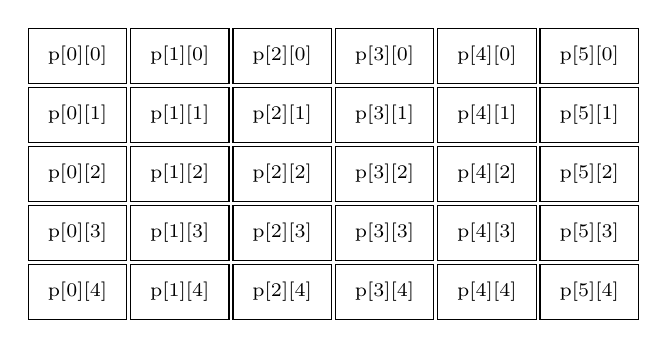
\begin{tikzpicture}[font=\scriptsize]
	\foreach \xi in {0,...,5}
		\foreach \yi in {0,...,4}
			\node[draw, minimum width=1.25cm, minimum height=0.7cm]
			at (1.3*\xi, -0.75*\yi) {p[\xi][\yi]};
\end{tikzpicture}
\end{center}

Die Breite des Bildes ist \texttt{p.length}, die Höhe ist \texttt{p[0].length}. Damit liegt $x$ im Bereich $0$ bis \texttt{p.length-1} und $y$ im Bereich $0$ bis \texttt{p[0].length-1}. Der Wert $0$ steht für die Farbe schwarz.

Schreiben Sie eine Klassenmethode \texttt{f}, die alle Pixel \textbf{außerhalb} eines Kreises schwarz färbt. Der Mittelpunkt des Kreises soll die Position $(171,161)$ haben, der Radius soll $130$ Pixel betragen. Alle Pixel, deren Abstand zum Mittelpunkt \textbf{größer} als $130$ Pixel ist, sollen auf $0$ gesetzt werden; die Pixel innerhalb des Kreises bleiben unverändert. Die Methode \texttt{f} soll als Parameter \texttt{p} einen zweidimensionalen \texttt{int}-Array haben und keinen Rückgabewert.

\begin{center}
\begin{tabular}{cc}
	
\includegraphics[width=0.34\textwidth]{../images/MyPicture.jpg} &
	
\includegraphics[width=0.34\textwidth]{../images/exam5_result.png} \\[0.3em]
	{\small\itshape Originalbild} & {\small\itshape Zielbild nach Aufruf von \texttt{f(p)}} \\
\end{tabular}
\end{center}

% =============================================
\clearpage
\section*{Aufgabe 2: Syntaxfehler -- Klassen A und B \hfill (20 Punkte)}

Der Programmcode der beiden Klassen \texttt{A} und \texttt{B} enthält mehrere syntaktische Fehler. Geben Sie zu jedem Fehler die Zeilennummer der Zeile an, in der sich der Fehler befindet, und beschreiben Sie jeweils den Fehler.

\begin{lstlisting}
public class A {

    public static int quadrat(int x) {
        return x * x;
    }

    public static void zeige(String t) {
        System.out.println(t)
    }
}

public class B {

    public int zaehler;

    public static int doppelt(int n) {
        return 2 * n;
    }

    public static boolean test(int n) {
        if (n > 0)
            return true;
        else if (n < 0)
            return false;
    }

    public static void main(String[] args) {
        int q = A.quadrat(3);
        A.zeige(q);
        zaehler = 0;
        int d = doppelt();
        boolean t = test(5);
        System.out.println(t)
    }
}
\end{lstlisting}

\begin{center}
\begin{tabular}{|p{1.6cm}|p{10.5cm}|}
	\hline
	\textbf{Zeile} & \textbf{Fehler} \\ \hline
	& \\[2cm] \hline
	& \\[2cm] \hline
	& \\[2cm] \hline
	& \\[2cm] \hline
	& \\[2cm] \hline
\end{tabular}
\end{center}

% =============================================
\clearpage
\section*{Aufgabe 3: Programmausgabe -- Rekursion über einen String \hfill (20 Punkte)}

Zu welcher Ausgabe kommt es, wenn man die Methode \texttt{main} der Klasse \texttt{X} ausführt?

\begin{lstlisting}
public class X {

    public static void f(String s, int i) {
        if (i >= s.length())
            return;
        f(s, i + 1);
        System.out.print(s.charAt(i));
    }

    public static void main(String[] args) {
        f("ABCD", 0);
        System.out.println();
        f("Hund", 1);
        System.out.println();
    }
}
\end{lstlisting}

\begin{hinweis}[Hinweis]
	\texttt{s.charAt(i)} liefert das $i$-te Zeichen des Strings \texttt{s}; \texttt{s.length()} liefert dessen Länge. \texttt{System.out.print} erzeugt keine, \texttt{System.out.println()} erzeugt einen Zeilenumbruch.
\end{hinweis}

\begin{hinweis}[Empfehlung]
	Achten Sie auf die Reihenfolge: Der rekursive Aufruf steht \emph{vor} der Ausgabeanweisung.
\end{hinweis}

% =============================================
\clearpage
\section*{Aufgabe 4: Methode implementieren -- Liste summieren \hfill (25 Punkte)}

Gegeben ist die folgende Klasse \texttt{Listenelement}:

\begin{lstlisting}
public class Listenelement {
    public int wert;
    public Listenelement nachfolger;

    public Listenelement(int wert) {
        this.wert = wert;
        nachfolger = null;
    }
}
\end{lstlisting}

Schreiben Sie zu der Klasse \texttt{Listenelement} eine \textbf{Objektmethode} mit dem Namen \texttt{summe}, die keinen Parameter hat und einen Rückgabewert vom Typ \texttt{int}. Die Methode \texttt{summe} soll die \textbf{Summe aller Werte} der Liste ab dem aufrufenden Listenelement (einschließlich) bestimmen und als Rückgabewert zurückgeben.

\begin{beispiel}[Beispiel]
	Besteht die Liste, auf deren erstem Element \texttt{summe} aufgerufen wird, aus den Werten $3$, $1$, $4$, so soll der Rückgabewert $8$ sein. Besteht sie nur aus einem einzigen Element mit dem Wert $7$, so soll der Rückgabewert $7$ sein.
\end{beispiel}

\end{document}
